\documentclass[]{scrartcl}
\title{Vorlesung Analysis II}
\usepackage{amsmath,amssymb,amsfonts}
\usepackage{stmaryrd}
\usepackage{mathtools}
\usepackage{latexsym}
\usepackage{graphicx}
\usepackage{tikz}
\usepackage{xcolor}
\usepackage{soul}
\usepackage{ upgreek }
\usepackage{hyperref}
\usepackage{tipa}
\usepackage[dvipsnames]{xcolor}
\hypersetup{
	colorlinks=true,
	linkcolor=blue,
	filecolor=magenta,      
	urlcolor=cyan,
	pdftitle={Overleaf Example},
	pdfpagemode=FullScreen,
}
\newcommand{\redcircle}[1]{%
	\tikz[baseline=(char.base)]{
		\node[shape=circle, draw=red, text=red, thick, inner sep=1pt] (char) 
		{\textbf{#1}};
	}%
}
\newcommand{\bluecircle}[1]{%
	\tikz[baseline=(char.base)]{
		\node[shape=circle, draw=blue, text=blue, thick, inner sep=1pt] (char) 
		{\textbf{#1}};
	}%
}
\newcommand{\blackcircle}[1]{%
	\tikz[baseline=(char.base)]{
		\node[shape=circle, draw=black, text=black, thick, inner sep=1pt] 
		(char) 
		{\textbf{#1}};
	}%
}
\setul{1pt}{3pt} % Linienhöhe und Abstand zum Text (optional anpassbar)

\setlength{\topmargin}{-.5in} \setlength{\textheight}{9.25in}
\setlength{\oddsidemargin}{0in} \setlength{\textwidth}{6.8in}
\setlength{\parindent}{0pt}

\begin{document}
\textbf{\underline{Teil 1: Differentialrechnung im $\mathbb{R}^n$}}\\
\\
\textbf{\underline{an6: Mittelwertsatz und der Satz von Schwarz}}\\
\\
\textbf{\underline{\underline{Stichworte:} MWS, stetig diff'bar, mehrfache 
partielle Ableitung, Satz von Schwarz}}\\
\\
\textbf{\underline{Literatur:}} \setulcolor{blue}\ul{[Hoff], Kapitel 9.5}\\
\\
\textbf{6.1. \underline{Einleitung:}} Der MWS wird für Skalarfelder 
verallgemeinert.\\
\\
\textbf{6.2. \underline{Erinnerung:}} Hatten der \setulcolor{red}\ul{MWS:} 
Vor.: $a,b \in \mathbb{R}, a\textless b, f:[a,b]\rightarrow \mathbb{R}$ stetig, 
in $]a,b[$ diff'bar.\\
Beh.: $\exists t\in]a,b[: f(b)-f(a)= f'(t)\cdot(b-a).$\\
Dies ist so \underline{nicht} übertragbar auf Abbildungen mit Werten in 
$\mathbb{R}^2$:\\
Betrachte $f:\mathbb{R}\rightarrow\mathbb{R}^2, t\rightarrow\begin{pmatrix}
	\cos t\\\sin t
\end{pmatrix}\in \mathbb{R}^2$ auf $[0,2\pi]$.\\
Aber: $ f(2\pi)-f(0)=0\neq\begin{pmatrix}
	-\sin t\\\cos t
\end{pmatrix}\cdot 2\pi$, da $||\begin{pmatrix}
	-\sin t\\\cos t
\end{pmatrix}||_2=1$ für alle $t\in\mathbb{R}.$\\
\\
\textbf{6.3. \underline{Konvention/Vereinbarung:}} Betrachte also nur 
\underline{$\mathbb{R}^{\textcolor{red}{1}}$}-wertige Funktion (d.h. 
Skalarfelder), die auf $U\subseteq \mathbb{R}$ definiert sind, wo jeder Punkt 
$a\in U$ innerer Punkt von U ist. Für je zwei Punkte $a,b\in U\subseteq 
\mathbb{R}^n$ sei weiter die (Verbindungs-)Strecke $\overline{ab}\subseteq U$, 
wobei \setulcolor{yellow}\ul{$\overline{ab}$}:=$\{a+t(b-a);t\in [0,1]\}$. U 
heißt dann \setulcolor{red}\ul{Konvex (Konvexe Menge).}\\
\begin{figure}[h]
	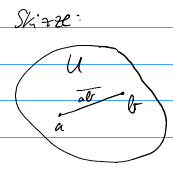
\includegraphics[width=3 cm,height=3cm]{bsp kap 6.3}
\end{figure}\\
\\
\textbf{6.4. \ul{Mittelwertsatz:}}\\
\underline{Vor.:} Sei $\overline{ab}\subseteq U\subseteq \mathbb{R}^n$ wie in 
\setulcolor{blue}\ul{6.3}, $f:U\rightarrow\mathbb{R}$ in allen Punkten von 
$\overline{ab}$ diff'bar.\\
\underline{Beh.:} \setulcolor{green}\ul{$\exists c \in 
\overline{ab}\backslash\{a,b\}$} mit \ul{$f(b)-f(a)=f'(c)\cdot(b-a)$} = 
$\textless f'(c)^T, b-a\textgreater.$\\
\underline{Bew.:} Setze \setulcolor{orange}\ul{$h(t):=f(a+t(b-a))$}, 
$h:[0,1]\rightarrow\mathbb{R}, t\rightarrowtail a +t(b-a)\xrightarrow{f} h(t).$ 
Werde auf h den alten \setulcolor{blue}\ul{MWS An12.13} an:\\
$\exists \xi \in ]0,1[$ mit $h(1)-h(0)=h'(\xi)(1-0) \Rightarrow f(b)-f(a)= 
f'(a+\xi(b-a))(b-a)=f'(c)\cdot(b-a)$\\
mit \setulcolor{orange}\ul{$c:=a+\xi\cdot(b-a)$} 
$\in\overline{ab}\backslash\{a,b\}$.\\
\strut\hfill$\square$\\
\textbf{6.5. \underline{Dies liefert folgende Möglichkeit zur 
Fehlerabschätzung:}}\\
Sei $b=a+\begin{pmatrix}
	\triangle\alpha_1\\\triangle\alpha_2\\\vdots\\\triangle\alpha_n
\end{pmatrix}\in\mathbb{R}^n.$\\
Dann gilt: 
$|f(b)-f(a)|=|f'(c)(b-a)|=|\sum_{j=1}^{n}D_jf(c)\triangle\alpha_j|\leq\sum_{j=1}^{n}
 S_j|\triangle\alpha_j|,$\\
 wenn $|D_jf(c)|\leq S_j$ mit $1\leq j\leq n$ ist.\\
 Dies ist u.U. eine grobe Abschätzung für die Abwechslung des WErts f(b) von 
 f(a).\\
 \\
 \textbf{6.6. \underline{Folgerung:}} \underline{Vor.:} Wie im 
 \setulcolor{blue}\ul{MWS 6.4.}, aber 
 $f:U\rightarrow$\setulcolor{green}\ul{$\mathbb{R}^m, \max_{1\leq i\leq 
 m}||f'(c)^T||_\infty \leq M\in \mathbb{R}_{\textgreater 0}$ für alle $c \in 
 \overline{ab}\backslash\{a,b\}$}.\\
 \underline{Beh.:} \ul{$||f(b)-f(a)||_\infty\leq nM\cdot||b-a||_\infty$}.\\
 \underline{Bew.:} Sei $i\in \{1,...,m\}$ so, dass $||f(b)-f(a)||_\infty = 
 |f_i(b)-f_i(a)|.$\\
 Mit dem \setulcolor{blue}\ul{MWS 6.4.} folgt: $\exists c \in 
 \overline{ab}\backslash\{a,b\}$ mit 
 $|f_i(b)-f_i(a)|=|\underbrace{f_i'(c)}_{\in \mathbb{R}^{1xm}}\cdot\underbrace{(b-a)}_{\in\mathbb{R}^n}|
  \leq ||f_i'(c)^T||_2\cdot||b-a||_2\leq nM\cdot ||b-a||_\infty.$\\
 \strut\hfill$\square$\\
 Dies Liefert und ein nützliches Kriterium zur Überprüfung der (totalen) 
 Differenzierbarkeit:\\
 \textbf{6.7. \underline{Satz:}} \underline{Vor.:}

















\end{document}